% !TEX TS-program = pdflatexmk
\documentclass[a4paper,11pt]{article}

\usepackage{Temp_short}
\usepackage[bottom]{footmisc}
\usepackage{commath}
\setlength{\jot}{0.3cm}
\allowdisplaybreaks[2]

\newenvironment{Ncenter}{%
  \setlength\topsep{-10pt}
  \setlength\parskip{-100pt}
  \begin{center}
}{%
  \end{center}
}

\bibliographystyle{abbrv}

\newcommand{\kmo}{k_{OT \to O+T}}
\newcommand{\ko}{k_{O+T \to OT}}
\newcommand{\kmt}{k_{OTE \to OT+E}}
\newcommand{\kt}{k_{OT+E \to OTE}}
\newcommand{\kc}{k_{OT+E \to OTE}}
\newcommand{\kE}{k_{OTE \to OCE}}
\newcommand{\kD}{k_{*C \to *+C}}
\newcommand{\vp}{v_{\mathrm{prod}}}
\newcommand{\vd}{v_{\mathrm{degrad}}}
\newcommand{\Trel}{T_{\rm{rel}}}
\newcommand{\Trelmin}{T_{\rm{rel,min}}}

\makeatletter 
\renewcommand{\thefigure}{S\@arabic\c@figure}
\renewcommand{\thesection}{S\@arabic\c@section}
\renewcommand{\thetable}{S\@arabic\c@table}
\addto\captionsenglish{\renewcommand{\figurename}{Supplementary Figure}}
\addto\captionsenglish{\renewcommand{\tablename}{Supplementary Table}}

\title{Supplementary File S1 for Pedersen et al. (2013), Nature Biotechnology}
\author{Lykke Pedersen, \and Peter H Hagedorn, \and Marie Lindholm, \and Morten Lindow}
\date{}

\usepackage{Sweave}
\begin{document}
\Sconcordance{concordance:SuppFile1.tex:SuppFile1.Rnw:%
1 47 1 1 0 8 1 1 2 1 0 2 1 3 0 1 2 14 1 1 4 3 0 1 1 6 0 1 2 1 1 1 30 7 %
1 1 14 1 46 13 1 1 2 1 0 1 3 2 0 1 3 2 0 1 1 1 3 2 0 1 2 1 0 1 1 1 2 1 %
0 1 1 1 2 1 0 1 1 1 2 1 0 1 1 1 2 1 0 1 1 1 2 1 0 1 1 1 2 1 0 1 1 1 2 1 %
0 1 1 1 3 5 0 1 2 8 1 1 7 12 1 1 3 2 0 1 1 1 4 3 0 1 1 1 3 5 0 1 19 11 %
1 1 2 8 0 2 2 1 0 2 1 3 0 1 18 32 1}

\maketitle

This document is the supplementary file for the manuscript entitled ``A kinetic model of enzyme recruiting oligonucleotides predicts an optimal affinity and thus explains why shorter and less affine oligonucleotides may be more potent" (2013) and a vignette for the R-package ASOmodel.


The functions and data used to produce the figures in the main manuscript and this supplementary file are available after installing and requiring the ASOmodel package in R
\begin{Schunk}
\begin{Sinput}
> require(devtools)
> install_github('ASOmodel',username='lykkep')
> require(ASOmodels)
\end{Sinput}
\end{Schunk}
The ASOmodels package contains the following functions:
\begin{enumerate}
\item \texttt{Trel}
\item \texttt{TrelNO}
\item \texttt{Trelstoc}
\item \texttt{plot.doseresponse}
\item \texttt{IC50}
\item \texttt{IC50NO}
\item \texttt{IC50stoc}
\item \texttt{diffASO}
\item \texttt{pretty10expLP}
\end{enumerate}

\newpage

\tableofcontents

\section{The rate-equations of the ASO model}
The kinetic ASO model governs eight ODEs for the seven variables: free target ($T$), free oligonucleotide ($O$), free RNAse H ($E$), complex of oligonucleotide and target ($OT$), complex of oligonucleotide, target and RNAse H  ($OTE$), complex of cleaved target, oligonucleotide and RNase H ($OCE$), and complex of cleaved target and oligonucleotide  ($OC$). The ASO model is described by the seven equations
\begin{align}
%T
\frac{\dif [T]}{\dif t} &= \vp - \vd [T]-k_{O+T \to OT} [T] [O] +k_{OT\to O+T } [OT] \\
%OT
\frac{\dif [OT]}{\dif t} &= \ko[O][T]-\kmo[OT] \nonumber \\
	& \quad -\kt[OT][E]+\kmt [OTE]-\vd[OT] \\
%OTE
\frac{\dif [OTE]}{\dif t} &= \kt[E][OT]-\kmt[OTE] \nonumber \\
	& \quad -(\vd+\kE)[OTE]\\
%E
\frac{\dif [E]}{\dif t} &= -\kt[E][OT]+\kmt([OTE]+[OCE]) \nonumber \\
	& \quad+\vd[OTE]\\
%O
\frac{\dif [O]}{\dif t}&= \kmo [OT]-\ko[O][T] \nonumber \\
	& \quad +\kD [OC]+\vd([OT]+[OTE])  \\
%ODE
\frac{\dif [OCE]}{\dif t}& = \kE [OTE]-\kmt [OCE]-\kD [OCE] \\
%OD
\frac{\dif [OC]}{\dif t}& = \kmt [OCE]-\kD [OC]
\end{align}
Complex formation and breaking are denoted by rate constants $k$ with subscripts. Target production and degradation rates are denoted by $\vp$ and $\vd$, respectively. The default parameter values are listed in Table~\ref{tb::par}.


Steady-state is reached when the Eqs.~(1)-(8) are equated to zero. Using Maple16 the steady-state concentrations are found. They all depend on the roots to a fourth order polynomial with coefficients calculated within the function \texttt{Trel()}. The one root that ensures that all concentrations are non-negative and also fullfills that
\begin{align*}
 &[O]+[OTE]+[OT]+[OCE]+[OC] = O_t \quad \mathrm{and}\\ 
 &[OTE]+[OCE]+[E] = E_t \enspace,
\end{align*}
is chosen. 

%Trel
When there is no oligonucleotide added to the system, then the steady-state concentration of target is $[T]=\frac{\vp}{ \vd}$. When oligonucleotide is added to the system then the total concentration of target at steady-state is the sum of the concentrations $[T]$, $[OT]$ and $[OTE]$. The relative total target concentration at steady-state is then calculated as 
\begin{equation}
\Trel = \frac{[T]+[OT]+[OTE]}{\frac{\vp}{ \vd}} \enspace.
\end{equation}

%IC50
The half maximal inhibitory concentration ($IC_{50}$) is the concentration of total nucleotide needed to inhibit the target concentration by half. The $IC_{50}$ is a measure of the potency of an oligonucleotide. A more potent oligonucleotide will have a lower $IC_{50}$ value. In mathematical terms the $IC_{50}$ value is defined as
\begin{equation}
IC_{50} = \left(O_t \left|\, \Trel = \frac{\mathrm{Eff}}{2}+\Trelmin \right.\right)  \enspace, \label{eq::IC50}
\end{equation}
where the efficacy (Eff, the maximum decrease in $\Trel$), and the minimum value of $\Trel$ ($\Trelmin$) are defined by
\begin{equation}
\textrm{Eff}=1-\lim_{O_t \to \infty} \Trel =1 - \Trelmin \label{eq:Eff} \enspace.
\end{equation}


\newpage
\section{Supplementary Table S1}
\begin{table}[!h]
\caption{Default values for the parameter-space of the ASO model. Concentrations are measured in $nM$ and time in $min$.}\label{tb::par}
\setlength\extrarowheight{5pt}  %Increases the height of each row
\begin{tabular}{| l | l | r | r |}
\hline
Parameter & Description &Default value & Ref  \\
\hline
$E_t$ & Total RNAse H conc & 1 nM & Ref. \cite{Amirkhanov:2002vo}\\
$O_t$ & Total oligo concentration & $\mathcal{O}(\mu M )$ & {}\\
$v_{prod}$ & Production of target & 0.2 nM/min & Ref. \cite{lodish2008molecular}\\
$v_{degrad}$ & Degradation of target & 0.04 $\rm{min}^{-1}$ & Ref. \cite{Yang:2003ja}\\
$D_{OT}$ & Dissociation constant of $OT$ & 0.3 nM & Ref. \cite{Christensen:2001te} \\
$D_{OTE}$ & Dissociation constant of $OTE$  & 70 nM & Ref. \cite{Amirkhanov:2002vo} \\
$k_{O+T \to OT }$ & Rate of $O+T \to OT$ & $0.2 \, (\rm{nM \,min})^{-1}$ & Ref. \cite{Christensen:2001te}\\
$k_{OT+E \to OTE}$ & Rate of $OT+E \to OTE$  & 5 $(\rm{nM \,min})^{-1}$ & Ref. \cite{Amirkhanov:2002vo}\\
$k_{OTE \to OCE}$ & Rate of $OTE \to OCE$  & 8 $\rm{min}^{-1}$ & Ref. \cite{Amirkhanov:2002vo}\\
$\alpha$ & Ratio of $\frac{k_{OT \to O+T}}{k_{\mathrm{*C \to *+C}}} \le 1$ & 0.1  & {}\\
\hline
\end{tabular}
\end{table}
%%%%



\section{Supplementary Figure S1}
The R-function \texttt{Trel()} calculates $\Trel$ and takes $O_t$ and the set of parameters as input
\begin{Schunk}
\begin{Sinput}
> parms <- c(Et = 1,KdOT = 0.3,kOpT = 0.2,KdOTE = 70,kOTpE = 5,	
+            vprod = 0.2,vdegrad = 0.04,alpha=0.1,kcleav = 8)
> Trel(otot=1,param=parms)
\end{Sinput}
\begin{Soutput}
[1] 0.6538694
\end{Soutput}
\end{Schunk}
For a sequence of different oligonucleotide concentrations ($O_t$), $\Trel$ can be calculated for varying parameter values. From this a dose-response curve is obtained.  Figure~\ref{fig::Etot} shows the change in the dose-reponse curve as the parameters vary. The plots in Fig.~\ref{fig::Etot} are produced using \texttt{plot.doseresponse()}.
%%%% FIGURE
\begin{figure}[!t]
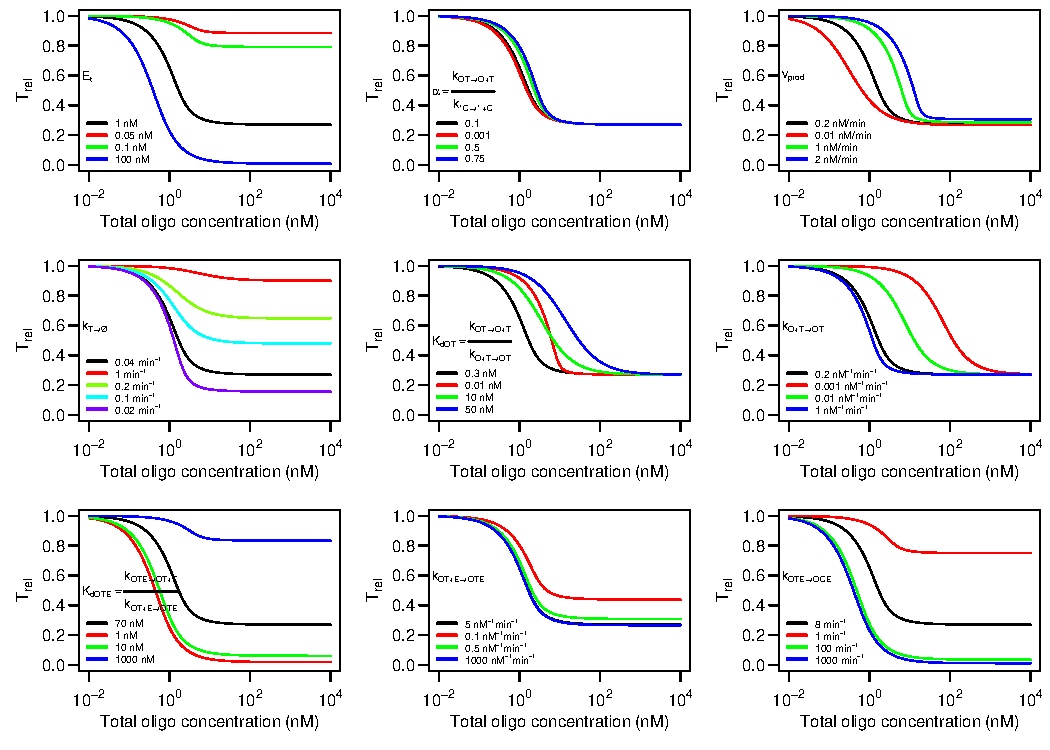
\includegraphics[width=\textwidth]{SuppFile1-S1.pdf}
\caption{Dose-response curves for different values of $E_{t}$, $\alpha$, $\vp$, $\vd$, $D_{OT}$, $\ko$, $D_{OTE}$, $\kt$, and $\kE$ (top,left to bottom,right). Black lines correspond to the parameter values listed in Supplementary Table \ref{tb::par}.}\label{fig::Etot}
\end{figure}

\section{Supplementary Figure S2}
Using the R-function \texttt{drm()} from the drc package (v2.3-0) a dose-response curve is fitted to $\Trel$ as a function of $O_t$ to obtain an $IC_{50}$ value. This is calculated through the function \texttt{IC50()} that takes $K_{dOT}$ and the set of parameters as input:
\begin{Schunk}
\begin{Sinput}
> IC50(KdOT=0.1,param=parms)
\end{Sinput}
\begin{Soutput}
    IC50 
1.218908 
\end{Soutput}
\end{Schunk}
 For a sequence of $K_{dOT}$ values one can calculate the corresponding $IC_{50}$ values and obtain Fig.~2c from the main manuscript, see Main Figure vignette. Figure \ref{fig::Opt} shows $IC_{50}$ as a function of $K_{dOT}$ for various parameter values. It can be seen that the optimum affinity, quantified by $K_{dOT}$, changes as parameters are changed. A larger value of $K_{dOT}$ correponds to a better affinity for the oligonucleotide.
% %
% <<S2,echo=FALSE,fig=TRUE,include=FALSE,width=7,height=4>>=
% parc <- c('Et','alpha','vprod','KdOTE','kcleav','vdegrad')
% xlabl <- list(~nM,~phantom(0),~'nM/min',~nM,'/min','/min')
% xlabll <- list(~E[t],~alpha,~v[prod],~D[OTE],~k[OTE%->%OCE],~v[degrad])
% parRange <- list(etot=c(0.01,1,10),alpha=c(0.005,0.01,0.95),
%                   vt=c(0.001,0.01,1.5),D2=c(0.5,10,100),
%                  kE=c(5,100,200),kd=c(0.005,0.05,0.5)) 
% D1_seq <- 10^seq(-3,3,by=0.25)
% IC50_fit <- as.list(1:length(parc))
% for(j in 1:length(parc)){
%  Lparseq <- parRange[[j]]
%  IC50_fit[[j]] <- matrix(NA, nrow=length(Lparseq),ncol=length(D1_seq))
%  
%  for(i in 1:length(Lparseq)){
%    parmsb <- parms; parmsb[parc[j]] <- Lparseq[i]
%    IC50_fit[[j]][i,] <- sapply(D1_seq,IC50,param=parmsb)
%  }
% }
% cbar <- c('orange','darkgreen','black')
% pdf('SuppFile1-S2.pdf',width=7,height=4)
% layout(matrix(c(1:6),2,3,byrow=T))
% for(j in 1:6){
%  Lparseq <- parRange[[j]]
% 
%  par(cex=0.75,mar=c(4,4,0.5,0.5),bty='o',mgp=c(2.2,0.7,0))
%  
%  for(i in 1:length(Lparseq)){
%    if(i==1){
%      plot(D1_seq,IC50_fit[[j]][1,],log='xy',panel.first=grid(col='grey',lty=3),
%            ylab=expression(IC[50]~' (nM)'),col=cbar[i],
%            ylim=c(1E-1,200),type='l',xaxt='n',yaxt='n',lwd=2,xlab=expression(K[dOT]~'(nM)'))
%      axis(1,at=c(1E-2,1,1E2),labels=pretty10expLP(10^c(-2,0,2),drop.1=T))
%      axis(2,at=c(1E-1,1,10,1E2),labels=pretty10expLP(10^c(-1:2),drop.1=T))
%    }else{
%      lines(D1_seq,IC50_fit[[j]][i,],col=cbar[i],lwd=2)
%     }
%   }
%   legend('bottomright',fill=cbar,cex=0.65,bg='white',x.intersp=0.2,
%           legend=as.expression(sapply(Lparseq,
%                            function(x) substitute(x*y,list(x=x,y=xlabl[[j]])))),
%           border=cbar,bty='o',box.lwd=0.5)
%   legend('top',as.expression(xlabll[[j]]),bty='n')
% }
% dev.off()
% @
% 

\begin{figure}[!h]
\begin{Ncenter}
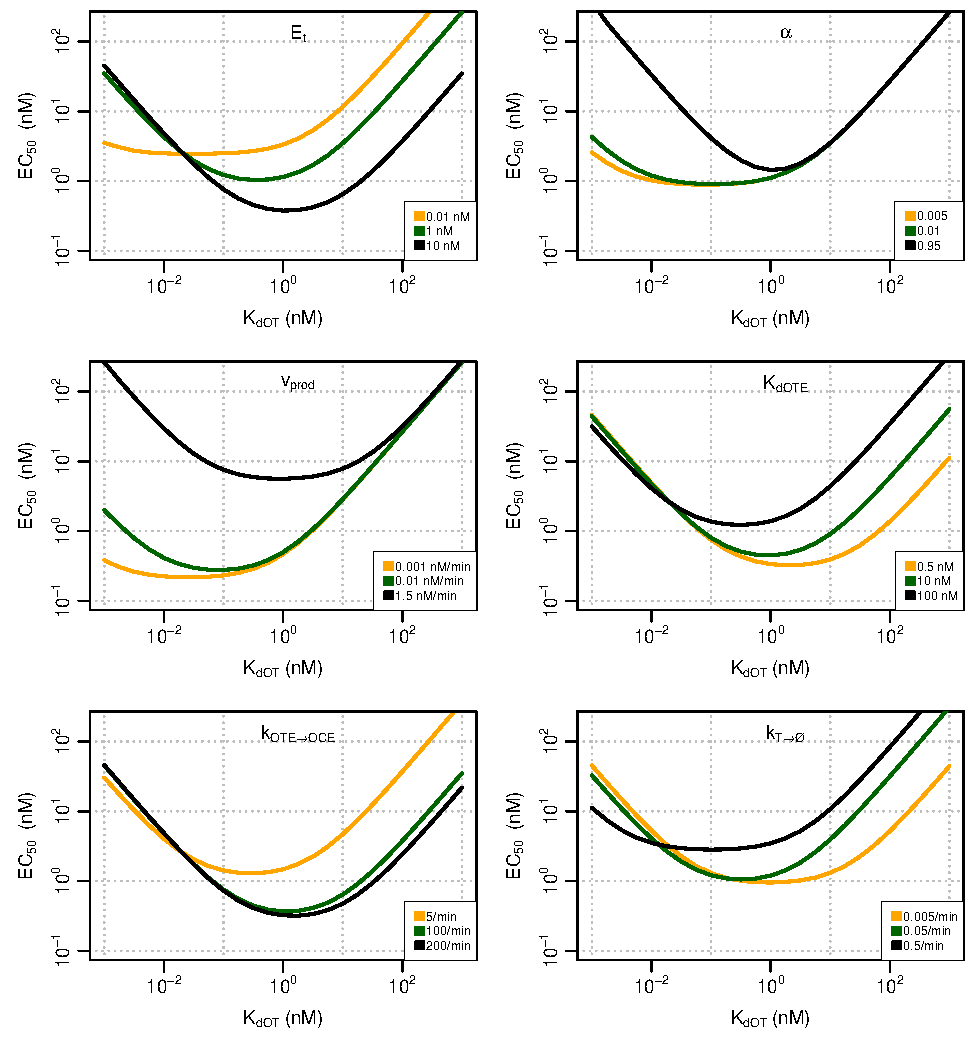
\includegraphics[width=\textwidth]{SuppFile1-S2.pdf}
\end{Ncenter}
\caption{The optimum affinity is dependent on the parameter settings. In the panels the $IC_{50}$ concentration is plotted against the binding affinity quantified by $K_{dOT}$ for various parameters. From top-left to bottom-right we have varied the total RNAse H concentration ($E_t$), alpha, the rate of target cleavage ($k_{OTE \to OCE}$), the target production ($v_{prod}$) and degradation ($v_{degrad}$), and the dissociation constant for the OTE complex ($D_{OTE}$).}\label{fig::Opt}
\end{figure}


\section{Supplementary Figure S3}
The stochastic simulation of the ASOmodel is carried out by use of the \texttt{ssa()} function from the GillespieSSA package (v.0.5-4). The inputs of ssa are an initial state vector (x0), which is the initial number of molecules, a propensity vector (a), which denotes the different states of the system, a state-change matrix (nu), which is the change in number of molecule (rows) if a reaction occur (column), the model-parameters (parms) and the final time (tf).
\begin{Schunk}
\begin{Sinput}
> library(GillespieSSA)
> parms1 <- c(k1 = 2E-5,k2 =50E-5 ,vt = 150,  kd = 0.04,		  
+               kE = 2, km1 =0.06, km2=2, k3 = 0.1)
> x0 <- c(Tt=parms1["vt"]/parms1["kd"],
+         OT=0,OTE=0,E=1e3,O=1e5,OCE=0,OC=0)
> names(x0) <- c('Tt','OT','OTE','E','O','OCE','OC')
> a <-  c("vt","k1*O*Tt","kd*Tt","km1*OT","km2*OTE","kd*OT",
+         "k2*OT*E","kd*OTE","kE*OTE","k3*OC","km2*OCE" )
> nu <- matrix(0,7,length(a))
> dimnames(nu) <- list(names(x0),a)
> #T
> nu['Tt',c('vt','km1*OT')] <- 1
> nu['Tt',c('k1*O*Tt','kd*Tt')] <- -1 
> #OT
> nu['OT',c('k1*O*Tt','km2*OTE')] <- 1
> nu['OT',c('km1*OT','k2*OT*E','kd*OT')] <- -1
> #OTE
> nu['OTE',c('k2*OT*E')] <- 1
> nu['OTE',c('km2*OTE','kd*OTE','kE*OTE')] <- -1
> #E
> nu['E',c('km2*OTE','kd*OTE','km2*OCE')] <- 1
> nu['E',c('k2*OT*E')] <- -1
> #O
> nu['O',c('km1*OT','kd*OTE','kd*OTE','kd*OT','k3*OC')] <- 1
> nu['O',c('k1*O*Tt')] <- -1
> #OCE
> nu['OCE',c('kE*OTE')] <- 1
> nu['OCE',c('km2*OCE')] <- -1
> #OC
> nu['OC',c('km2*OCE')] <- 1
> nu['OC',c('k3*OC')] <- -1
> Gillespie <- ssa( x0=x0,# initial state vector
+       a=a, # propensity vector
+       nu=nu, # state-change matrix
+       parms = parms1, # model parameters
+       tf=1E3, # final time
+       method = "ETL" # SSA method
+ )
\end{Sinput}
\end{Schunk}
Check that $[O]+[OT]+[OTE]+[OCE]+[OC] = O_t$ at all times:
\begin{Schunk}
\begin{Sinput}
> range(rowSums(Gillespie$data[,c('O','OT','OTE','OCE','OC')])-
+         x0['O'])
\end{Sinput}
\begin{Soutput}
[1] 0 0
\end{Soutput}
\end{Schunk}
Check that $[E]+[OTE]+[OCE] = E_t$ at all times:
\begin{Schunk}
\begin{Sinput}
> range(rowSums(Gillespie$data[,c('OTE','OCE','E')])-x0['E'])
\end{Sinput}
\begin{Soutput}
[1] 0 0
\end{Soutput}
\end{Schunk}
Supplementary Figure S3 shows $\Trel$, from the Gillespie simulation, as a function of time.
\begin{figure}[!h]
\begin{Ncenter}
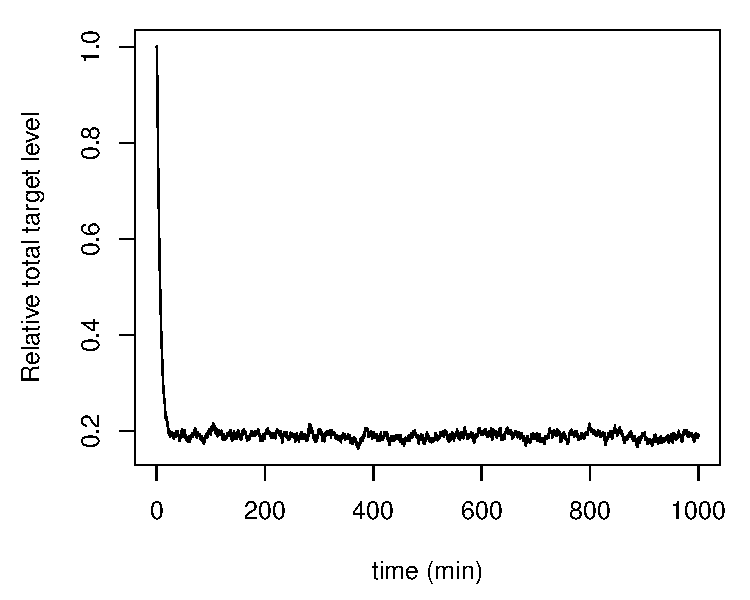
\includegraphics[width=0.6\textwidth]{SuppFile1-Trel.pdf}
\end{Ncenter}
\caption{The time-trace for the relative total target level.}\label{fig:Trel}
\end{figure}

\section{Supplementary Figure S4}
After a while the relative target concentration reaches a plateau. In Supplementary Figure S3 the plateu starts around $50min$. The mean of $\Trel$ within the plateu is calculated through the function \texttt{Trelstoc()}. Using this function we can generate dose-response curves (Supplementary Figure S4,left). From these the $IC_{50}$ values can be calculated using the \texttt{IC50stoc()} function and subsequently plotted as a function of $\kmo$ (Supplementary Figure S4,right).
\begin{Schunk}
\begin{Sinput}
> lseq <- c(1,2.5,5,7.5)
> #### Sequence of k(OT -> O+T) values
> KM <- c(1E-3*lseq[-1],1E-2*lseq,1E-1*lseq)
> #### Generation of dose-response curves
> DRcurve <- lapply(KM,function(kmi){ 
+             sapply(10^seq(2.5,6,by=0.2),
+                    function(i) Trelstoc(i,km1=kmi)$Tstat)})
> DRc <- lapply(DRcurve,function(x) x[,!is.na(x[3,])] )
> #### Calculation of IC50
> IC50_KM <- sapply(1:length(DRc),
+               function(x){IC50stoc(DRc[[x]][2,],DRc[[x]][1,])})
\end{Sinput}
\end{Schunk}
\begin{figure}[!h]
\begin{Ncenter}
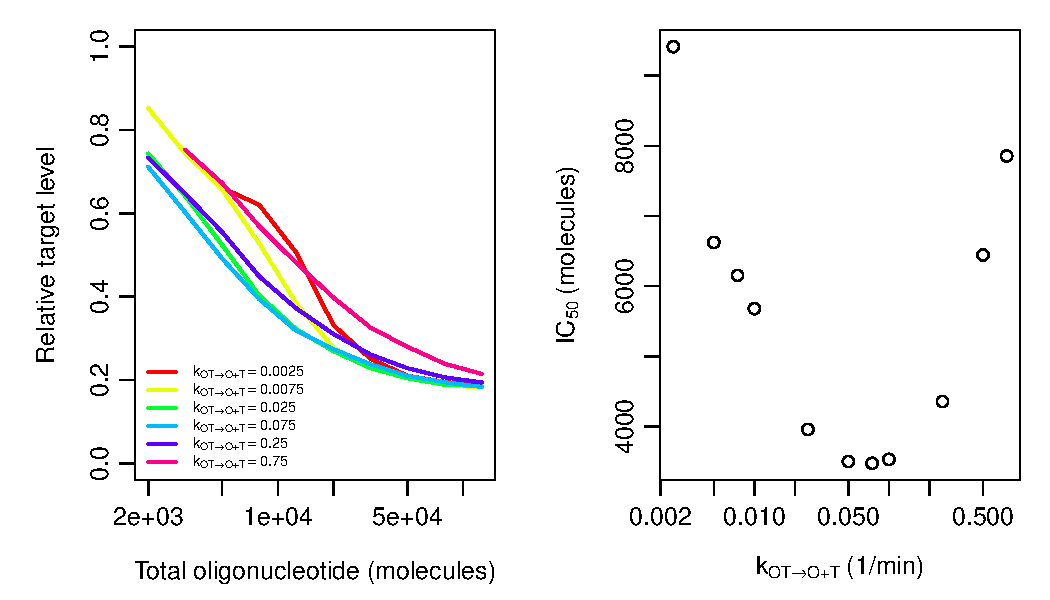
\includegraphics[width=\textwidth]{SuppFile1-IC50.pdf}
\end{Ncenter}
\caption{Left: Dose-response curves for various values of $\kmo$. Right: The $IC_{50}$-value as a function of $\kmo$.}\label{fig:figIC50}
\end{figure}
\newpage

%%%%%%%%%%%%%%%%%%%%%%%%%%%%%%%%%%%%%%%%%%%%%%%%%%%
\section{Supplementary Figure S5}
\begin{figure}[!h]
\begin{Ncenter}
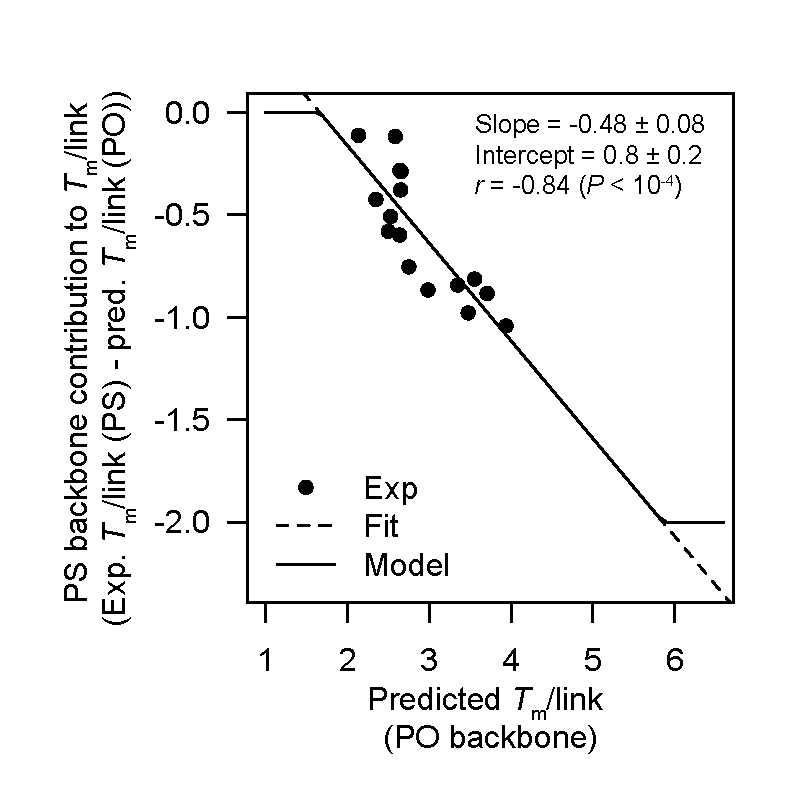
\includegraphics[width=0.65\textwidth]{SuppFig_PS.pdf}
\end{Ncenter}
\caption{The effect on $T_m$ of a phosphorothioate backbone was estimated using published data from Ref. \cite{Hashem:1998kf}.}\label{fig:figPS}
\end{figure}

\section{Supplementary Figure S6}
\begin{figure}[!h]
\begin{Ncenter}
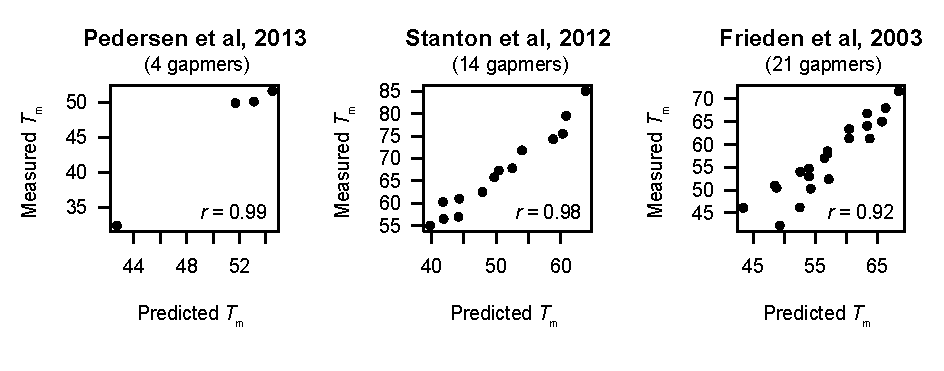
\includegraphics[width=\textwidth]{SuppFigS3.pdf}
\end{Ncenter}
\caption{Measured melting temperature vs predicted melting temperatur. There are clear correlations (r > 0.92, P < 0.01, Pearson's correlation) between predicted and measured $T_m$. Pedersen et al: 4 LNA-modified oligonucleotides targeting apolipoprotein B (this work), Stanton et al: 14 LNA-modified oligonucleotides targeting the glucocorticoid receptor \cite{Stanton:2012fu}. Frieden et al: 21 LNA-modified oligonucleotides targeting the luciferase firefly gene \cite{Frieden:2003er}.}\label{fig:figTm}
\end{figure}

\newpage
\bibliography{ASOmodels}


\end{document}
